% LaTeX report template 
%

% This is a comment: in LaTeX everything that in a line comes
% after a "%" symbol is treated as comment

\documentclass[11pt, a4paper]{article}
\usepackage{graphicx}
\usepackage{amsmath}
\usepackage{listings}


\title{Assignment 5} % Title

\author{Om Shri Prasath (EE17B113)} % Author name

\date{\today} % Date for the report
\begin{document}	
	
\maketitle % Insert the title, author and date		
  \section{Introduction}
  This report will discuss about the solver for the currents in a
resistor and discusses about the current's dependency on the shape of
the resistor and also discusses which part of the resistor is likely to
get hottest.Here we analyse the currents in a square copper plate to
which a wire is soldered to the middle of it.It also discuss about how
to find stopping condition for the solver after certain iterations,and
to model the errors obtained using Least Squares after analysing the
actual errors in semilog and loglog plots.And finally we find the
currents in the resistor after applying boundary conditions and analyse
the vector plot of current flow and conclude which part of resistor will
become hot.

	\begin{itemize}
    \item
      A wire is soldered to the middle of a copper plate and its voltage is
      held at 1 Volt. One side of the plate is rounded, while the remaining
      are floating. The pblate is 1 cm by 1 cm in size.
    \item
      To solve for currents in resistor,we use following equations and
      boundary conditions mentioned below:
    \item
      Conductivity (Differential form of ohm's law)
    \end{itemize}
    
    \begin{equation}
    \vec{J} = \sigma\vec{E}
       \end{equation}
    
    \begin{itemize}
    \item
      Electric field is the gradient of the potential
    \end{itemize}
    
    \begin{equation}
    \vec{E} = -\nabla{\phi}
       \end{equation}
    
    \begin{itemize}
    \item
      Charge Continuity equation is used to conserve the inflow and outflow
      charges
    \end{itemize}
    
    \begin{equation}
    \nabla.\vec{J} = -\frac{\partial \rho}{\partial t}
       \end{equation}
    
    \begin{itemize}
    \item
      Combining the above equations above, we get
    \end{itemize}
    
    \begin{equation}
    \nabla.(-\sigma\nabla\phi) = -\frac{\partial \rho}{\partial t}
       \end{equation}
    
    \begin{itemize}
    \item
      Assuming that our resistor contains a material of constant
      conductivity, the equation becomes
    \end{itemize}
    
    \begin{equation}
    \nabla^{2}\phi = \frac{1}{\sigma}\frac{\partial \rho}{\partial t}
       \end{equation}
    
    \begin{itemize}
    \item
      For DC currents, the right side is zero, and we obtain
    \end{itemize}
    
    \begin{equation}
    \nabla^{2}\phi = 0
       \end{equation}
    
    \begin{itemize}
    \item
      Here we use a 2-D plate so the Numerical solutions in 2D can be easily
      transformed into a difference equation. The equation can be written
      out in
    \end{itemize}
    
    \begin{equation}
    \frac{\partial^{2} \phi}{\partial x^{2}}+ \frac{\partial^{2} \phi}{\partial y^{2}} = 0
     \end{equation}
    
    \begin{equation}
    \frac{\partial \phi}{\partial x}_{(x_i,y_j)} = \frac{\phi(x_{i+1/2},y_j) - \phi(x_{i-1/2},y_j)}{\Delta x}
     \end{equation}
    
    \begin{equation}
    \frac{\partial^{2} \phi}{\partial x^{2}}_{(x_i,y_j)} = \frac{\phi(x_{i+1},y_j) -2\phi(x_i,y_j)+ \phi(x_{i-1},y_j)}{(\Delta x)^{2}}
     \end{equation}
    
    \begin{itemize}
    \item
      Using above equations we get
    \end{itemize}
    
    \begin{equation}
            \phi_{i,j} = \frac{\phi_{i+1,j} + \phi_{i-1,j} + \phi_{i,j+1} + \phi_{i,j-1}}{4} 
    \end{equation}
    
    \begin{itemize}
    \item
      Thus, the potential at any point should be the average of its
      neighbours. This is a very general result and the above calculation is
      just a special case of it. So the solution process is to take each
      point and replace the potential by the average of its neighbours. Keep
      iterating till the solution converges (i.e., the maximum change in
      elements of \(\phi\) which is denoted by \(error_k\) in the code
      ,where 'k' is the no of iteration, is less than some tolerance which
      is taken as \(10^{-8}\)).
    \item
      At boundaries where the electrode is present, just put the value of
      potential itself. At boundaries where there is no electrode, the
      current should be tangential because charge can't leap out of the
      material into air. Since current is proportional to the Electric
      Field, what this means is the gradient of \(\phi\) should be
      tangential. This is implemented by requiring that \(\phi\) should not
      vary in the normal direction
    \item
      At last we solve for currents in the resistor using all these
      information!
  \end{itemize}

  \section{Python Code :}\label{python-code}
  \subsection{Question 1}\label{question-1}

\subsubsection{Part A}\label{part-a}

\begin{itemize}
\item
  Define the Parameters, The parameter values taken for my particular code were \(N_x = 50\) and \(N_y = 50\) and No of
  iterations : 6000
\item
  These values are taken to discuss about Stopping condition,etc
\item
  To allocate the potential array \(\phi = 0\) .Note that the array
  should have \(N_y\) rows and \(N_x\) columns.
\item
  To find the indices which lie inside the circle of radius 0.35 using
  meshgrid() by equation :
\end{itemize}

\begin{equation}
X ^2 +Y ^2 \leq	 0.35^2
\end{equation}

\begin{itemize}
\item
  Then assign 1 V to those indices.
\item
  To plot a contour plot of potential \(\phi\) and to mark V=1 region in
  red

\end{itemize}
\newpage
\textit{\textbf{Code:}}
\begin{lstlisting}
  Nx = 50  
  Ny = 50
  radius = 0.35
  Niter = 6000
  
  
  phi = np.zeros((Ny, Nx))
  y = linspace(-0.5, 0.5, Ny)
  x = linspace(-0.5, 0.5, Nx)

  X, Y = meshgrid(x, -y)           
  ii = where(square(X) + square(Y) <= pow(radius, 2))
  phi[ii] = 1.0 
  
  
  fig1 = figure()
  ax1 = fig1.add_subplot(111)
  plt1 = ax1.contourf(phi, cmap=cm.jet, clabel="$\phi$")
  title("Figure 1 : Contour Plot of $\phi$")
  ax = gca()
  fig1.colorbar(plt1, ax=ax, orientation='vertical')
  xlabel("$x$")
  ylabel("$y$")
  savefig("Figure1.jpg")
  show()
  
  
       \end{lstlisting}
       \newpage
	     \begin{figure}[!tbh]
        \centering
        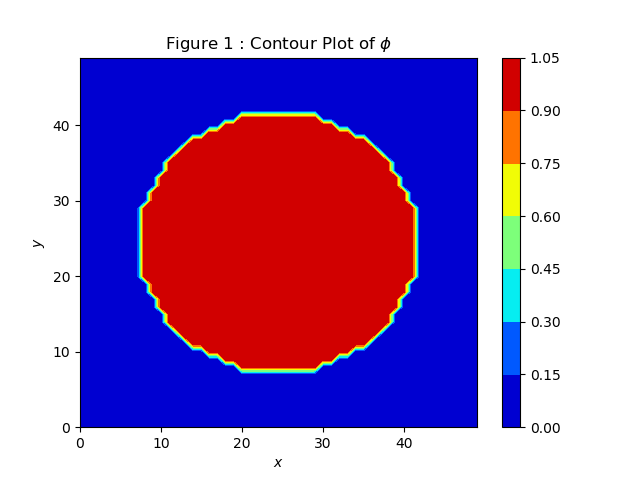
\includegraphics[scale=0.8]{./../Extras/Figure_1.png}  
        \caption{Contour plot of initial potential}
   \end{figure}
   \paragraph{Results and Discussion :}\label{results-and-discussion}

   \begin{itemize}
   \item
     The contour plot of potential becomes smoother i.e it almost becomes
     circular as we increase \(N_x\) and \(N_y\),because we get more no of
     points,so the potential gradient is smoothed out between adjacent
     points since there are more no of points
   \end{itemize}
   \newpage
   \subsubsection{Part B :}\label{part-b}

   \begin{itemize}
   \item
     To Perform the iterations
   \item
     To update the potential \(\phi\) according to Equation below using
     vectorized code
   \end{itemize}
   
   \begin{equation}
           \phi_{i,j} = \frac{\phi_{i+1,j} + \phi_{i-1,j} + \phi_{i,j+1} + \phi_{i,j-1}}{4} 
   \end{equation}
   
   \begin{itemize}
   \item
     To apply Boundary Conditions where there is no electrode, the gradient
     of \(\phi\) should be tangential. This is implemented by Equation
     given below , basically potential should not vary in the normal
     direction so we equate the last but row or column to outermost row or
     column correspondingly when applying boundary conditions for a side of
     plate,implemented using Vectorized code
   \end{itemize}
   
   \begin{equation}
    \frac{\partial \phi}{\partial n} = 0
   \end{equation}
   
   \begin{itemize}
   \item
     To plot the errors in semilog and loglog and observe how the errors
     are evolving.
   \end{itemize}

\textit{\textbf{Code:}}
   \begin{lstlisting}
    def createAmatrix(nrow, x):
    A = zeros((nrow, 2))  
    A[:, 0] = 1
    A[:, 1] = x
    return A

def fitForError(errors, x):
    A = createAmatrix(len(errors), x)
    return A, lstsq(A, log(errors), rcond=None)[0]

def computeErrorFit(M, c):
    return exp(M.dot(c))

errors = zeros(Niter)  
iterations = []  

for k in range(Niter):
    
    oldphi = phi.copy()

    phi[1:-1, 1:-1] = 0.25 * \
        (phi[1:-1, 0:-2]+phi[1:-1, 2:]+phi[0:-2, 1:-1]+phi[2:, 1:-1])

    phi[1:-1, 0] = phi[1:-1, 1]  
    phi[1:-1, -1] = phi[1:-1, -2]  
    phi[0, :] = phi[1, :]  
    
    phi[ii] = 1.0

    errors[k] = (abs(phi-oldphi)).max()
    iterations.append(k)

fig2 = figure()
ax2 = fig2.add_subplot(111)
ax2.semilogy(iterations, errors, 'g', 
                      markersize=8, label="Original Error")
ax2.legend()
title(r"Figure 2a : Error Vs No of iterations (Semilog)")
xlabel("$Niter$")
ylabel("Error")
grid()
savefig("Figure2a.jpg")
show()

fig2b = figure()
ax2b = fig2b.add_subplot(111)
ax2b.loglog(iterations, errors, 'g', 
                    markersize=8, label="Original Error")
ax2b.legend()
title(r"Figure 2b : Error Vs No of iterations (Loglog)")
xlabel("$Niter$")
ylabel("Error")
grid()
savefig("Figure2b.jpg")
show()
    
         \end{lstlisting}
     \newpage
     \begin{figure}[!tbh]
      \centering
      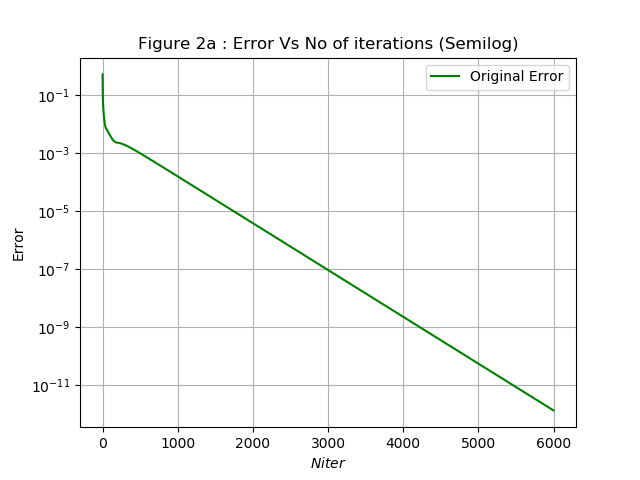
\includegraphics[scale=0.8]{./../Extras/Figure_2.png}  
      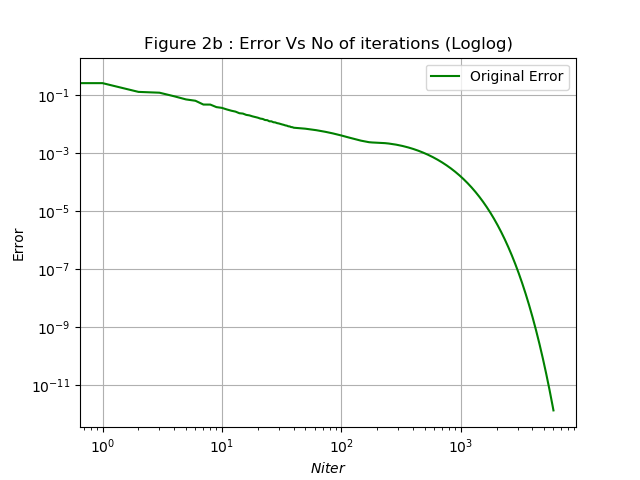
\includegraphics[scale=0.8]{./../Extras/Figure_3.png}  
      \caption{Normal and Log-Log plot of Error vs No.of Iterations}
 \end{figure}
 \newpage
 \paragraph{Results and Discussion:}\label{results-and-discussion}

 \begin{itemize}
 \item
   As we observe the Figure 2a that error decreases linearly for higher
   no of iterations,so from this we conclude that for large iterations
   error decreases exponentially with No of iterations i.e it follows
   \(Ae^{Bx}\) as it is a semilog plot
 \item
   And if we observe loglog plot the error is almost linearly decreasing
   for smaller no of iterations so it follows \(a^x\) form since it is
   loglog plot and follows some other pattern at larger iterations.
 \item
   So to conclude the error follows \(Ae^{Bx}\) for higher no of
   iterations(\(\approx\) 500) and it follows \(a^x\) form for smaller
   iterations which can be seen from figure 2a \& 2b respectively
 \end{itemize}
 \newpage

    \subsubsection{Part C :}\label{part-c}

\begin{itemize}
\item
  To find the fit using Least squares for all iterations named as
  \textbf{fit1}and for iterations \(\geq\) 500 named as \textbf{fit2}
  separately and compare them.
\item
  As we know that error follows \(Ae^{Bx}\) at large iterations, we use
  equation given below to fit the errors using least squares
\end{itemize}

\begin{equation}
    logy = logA + Bx
\end{equation}

\begin{itemize}
\item
  To find the time constant of error function obtained for the two cases
  using lstsq and compare them
\item
  To plot the two fits obtained and observe them
\end{itemize}

\textit{\textbf{Code:}}
   \begin{lstlisting}
M1, c1 = fitForError(errors, iterations)
M2, c2 = fitForError(errors[500:], iterations[500:])
print("Fit1 : A = %g , B = %g" % ((exp(c1[0]), c1[1])))
print("Fit2 : A = %g , B = %g" % ((exp(c2[0]), c2[1])))
print("The time Constant (1/B) all iterations considered:
 %g" % (abs(1/c1[1])))
print("The time Constant (1/B) for higher iterations (from 500) :
 %g" % (abs(1/c2[1])))
error_fit1 = computeErrorFit(M1, c1)
M2new = createAmatrix(len(errors), iterations)
error_fit2 = computeErrorFit(M2new, c2)
fig3 = figure()
ax3 = fig3.add_subplot(111)

ax3.semilogy(iterations[0::200], error_fit1[0::200],
             'ro', markersize=8, label="Fit1")
ax3.semilogy(iterations[0::200], error_fit2[0::200],
             'bo', markersize=6, label="Fit2")
ax3.semilogy(iterations, errors, 'k', markersize=6, label="Actual Error")
ax3.legend()
title(r"Figure 3 : Error Vs No of iterations (Semilog)")
xlabel("$Niter$")
ylabel("Error")
grid()
savefig("Figure3.jpg")
show()
 
\end{lstlisting}
\newpage
\begin{figure}[!tbh]
 \centering
 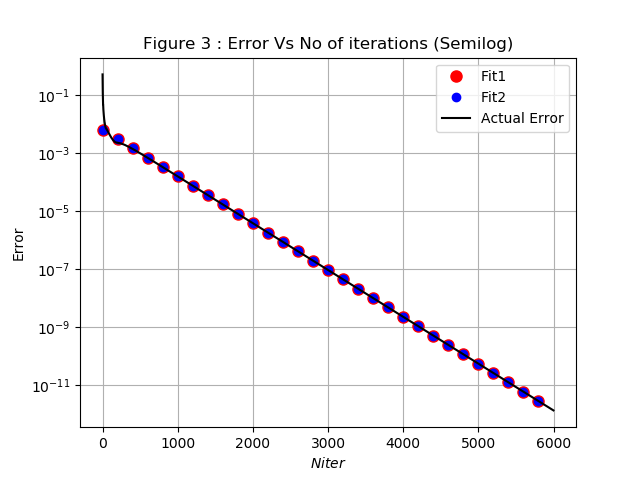
\includegraphics[scale=0.8]{./../Extras/Figure_4.png}  
 \caption{Semilog plot of Error vs No.of Iterations}
\end{figure}
\newpage
\paragraph{Results and Discussion:}\label{results-and-discussion}

\begin{itemize}
\item 
Fit1 : A = 0.00631664 , B = -0.00371103\newline
Fit2 : A = 0.00629419 , B = -0.00370997
\item
  As we observe the Fit1's time constant and Fit2's time constant,
  Fit2's is slightly higher than Fit1's time constant,so the error
  decreases slowly at larger iterations compared to fit1.
\item
  Ideally the time constant for Fit2 should be larger than Fit1 with
  good margin,since we take less no of points i.e stepsize \(N_x\) and
  \(N_y\) being less,we get less difference between their time
  constants,but if we increase the \(N_x\) and \(N_y\) to 100,100
  respectively I tried and got these results :

  \begin{itemize}
  \item
    Time Constant for Fit1 : 269.467s
  \item
    Time Constant for Fit2 (higher iterations from 500) : 269.544s
  \end{itemize}
\item
  As we see that there is a significance difference between them, since
  we increased the stepsize to 100!
\item
  So the time constant increase with increase in \(N_x\) and \(N_y\)
\end{itemize}
\newpage
\subsubsection{Stopping Condition :}\label{stopping-condition}

\begin{itemize}
\item
  To find the cumulative error for all iterations and compare them with
  some error tolerance to stop the iteration.
\item
  So to find the cumulative error, we add all the absolute values of
  errors for each iteration since worst case is, all errors add up
\item
  So we use the equations given below:
\end{itemize}

\begin{equation}
    Error = \sum_{N+1}^{\infty}error_k
  \end{equation}

\begin{itemize}
\item
  The above error is approximated to
\end{itemize}

\begin{equation}
    Error \approx -\frac{A}{B}exp(B(N+0.5))
    \end{equation}

where N is no of iteration

\textit{\textbf{Code:}}
\begin{lstlisting}
def cumerror(error, N, A, B):
return -(A/B)*exp(B*(N+0.5))

def findStopCondn(errors, Niter, error_tol):
  cum_error = []
  for n in range(1, Niter):
      cum_error.append(cumerror(errors[n], n, exp(c1[0]), c1[1]))
      if(cum_error[n-1] <= error_tol):
          print("last per-iteration change in the error is %g"
                % (cum_error[-1]-cum_error[-2]))
          return cum_error[n-1], n

  print("last per-iteration change in the error is %g"
        % (np.abs(cum_error[-1]-cum_error[-2])))
  return cum_error[-1], Niter

error_tol = pow(10, -8)
cum_error, Nstop = findStopCondn(errors, Niter, error_tol)
print("Stopping Condition N: %g and Error is %g" % (Nstop, cum_error))

\end{lstlisting}
\newpage
\paragraph{Results and Discussion :}\label{results-and-discussion}

\begin{itemize}
\item
  From running the code, we get stopping condition as N : 5107 and the total cumulative
  error till that iteration is \(9.98483*10^{-9}\)
\item
  And the last per iteration change in error: \(3.71228*10^{-11}\)
\item
  So we observe that the profile was changing very little every
  iteration, but it was continuously changing. So the cumulative error
  was still large.
\item
  So that is why this method of solving Laplace's Equation is known to
  be one of the worst available. This is because of the very slow
  coefficient with which the error reduces.
\end{itemize}
\subsubsection{Part D: Surface Plot of
Potential}\label{part-d-surface-plot-of-potential}

\begin{itemize}
\item
  To do a 3-D surface plot of the potential.
\item
  To plot contour plot of potential
\item
  And analyse them and to comment about flow of currents
\end{itemize}
\textit{\textbf{Code:}}
\begin{lstlisting}
  fig5 = figure()
  ax5 = p3.Axes3D(fig5)
  title("Figure 5: 3-D surface plot of the potential $\phi$")
  surf = ax5.plot_surface(X, Y, phi, rstride=1, cstride=1, cmap=cm.jet)
  ax5.set_xlabel('$x$')
  ax5.set_ylabel('$y$')
  ax5.set_zlabel('$z$')
  cax = fig5.add_axes([1, 0, 0.1, 1])
  savefig("Figure5.jpg")
  fig5.colorbar(surf, cax=cax, orientation='vertical')
  show()

  fig6 = figure()
  ax6 = fig6.add_subplot(111)
  plt6 = ax6.contourf(X, Y, phi, cmap=cm.jet)
  title("Figure 6 : Contour plot of Updated potential $\phi$")
  ax = gca()
  fig1.colorbar(plt6, ax=ax, orientation='vertical')
  xlabel("$x$")
  ylabel("$y$")
  grid()
  savefig("Figure6.jpg")
  show()

  \end{lstlisting}

\newpage
\begin{figure}[!tbh]
 \centering
 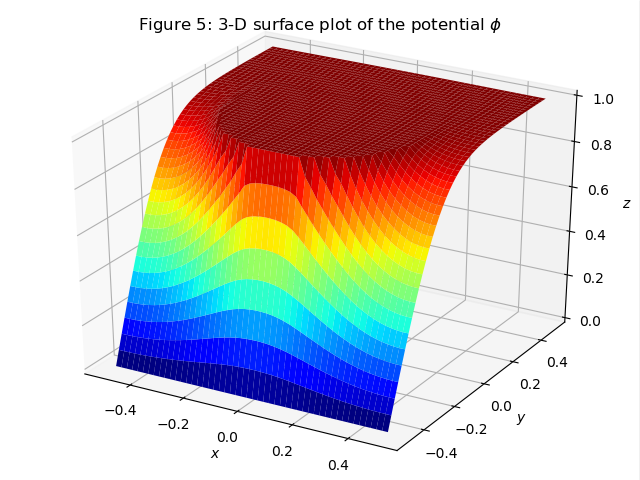
\includegraphics[scale=0.8]{./../Extras/Figure_5.png}  
 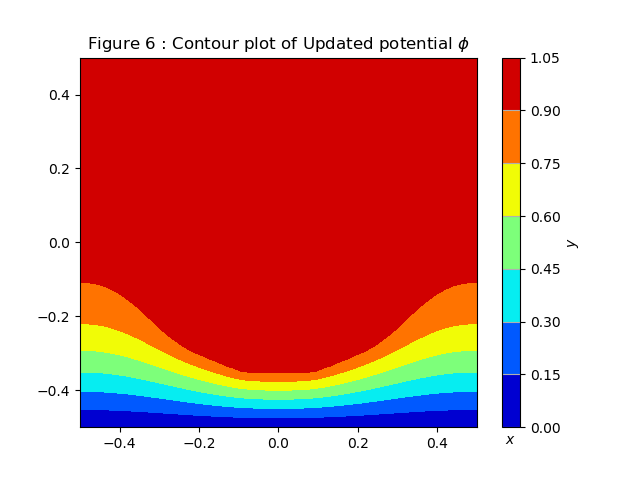
\includegraphics[scale=0.8]{./../Extras/Figure_6.png}  
 \caption{3-D Surface potential plot and Contour plot of potential}
\end{figure}
\newpage
\paragraph{Results and Discussion:}\label{results-and-discussion}

\begin{itemize}
\item
  As we observe that the surface plot we conclude that after updating
  the potential,the potential gradient is higher in down part of the
  plate since, the down side is grounded and the electrode is at 1 V,so
  there is high potential gradient from electrode to grounded plate.
\item
  And the upper part of the plate is almost 1 V since they didnt have
  forced Voltage and their's were floating,so while applying updating we
  replaced all points by average of surrounding points so the potential
  is almost 1 V in the upper region of the plate!
\item
  Same observation we see using contour plot in 2 dimensions, we note
  that there are gradients in down part of the plate and almost
  negligible gradient in upper part of the plate.
\end{itemize}
\newpage
\subsubsection{Part E : Vector Plot of Currents
:}\label{part-e-vector-plot-of-currents}

\begin{itemize}
\item
  To obtain the currents by computing the gradient.
\item
  The actual value of \(\sigma\) does not matter to the shape of the
  current profile, so we set it to unity. Our equations are
\end{itemize}

\begin{equation}
    J_x = -\frac{\partial \phi}{\partial x} 
  \end{equation}

\begin{equation}
    J_y = -\frac{\partial \phi}{\partial y} 
  \end{equation}

\begin{itemize}
\item
  To program this we use these equations as follows:
\end{itemize}

\begin{equation}
        J_{x,ij} = \frac{1}{2}(\phi_{i,j-1} - \phi_{i,j+1}) 
    \end{equation}

\begin{equation}
        J_{y,ij} = \frac{1}{2}(\phi_{i-1,j} - \phi_{i+1,j}) 
    \end{equation}
  
  \textit{\textbf{Code:}}
\begin{lstlisting}
  Jx = zeros((Ny, Nx))
  Jy = zeros((Ny, Nx))
  
  Jx[1:-1, 1:-1] = 0.5*(phi[1:-1, 0:-2] - phi[1:-1, 2:])
  Jy[1:-1, 1:-1] = 0.5*(phi[2:, 1:-1] - phi[0:-2, 1:-1])
  
  
  fig7 = figure()
  ax7 = fig7.add_subplot(111)
  
  ax7.scatter(x[ii[0]], y[ii[1]], color='r', s=12, label="V = 1 region")
  
  ax7.quiver(X, Y, Jx, Jy)
  ax7.set_xlabel('$x$')
  ax7.set_ylabel('$y$')
  
  ax7.legend()
  title("The Vector plot of the current flow")
  savefig("Figure7.jpg")
  show()

  \end{lstlisting}
  \newpage
  \begin{figure}[!tbh]
   \centering
   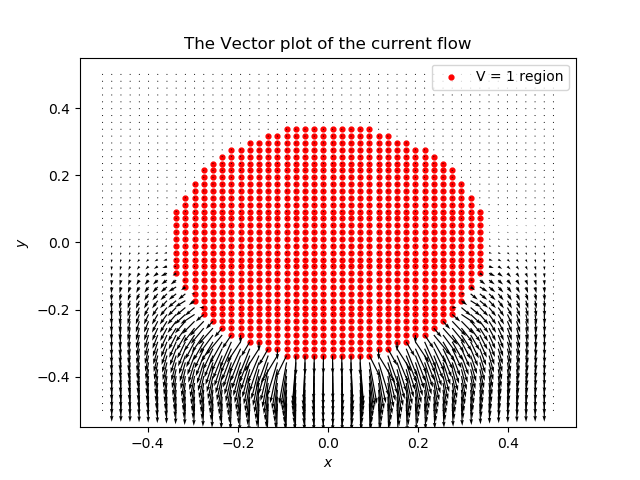
\includegraphics[scale=0.8]{./../Extras/Figure_7.png}  
   \caption{Vector plot of current flow}
  \end{figure}

  \newpage
  \paragraph{Results and Discussion:}\label{results-and-discussion}

  \begin{itemize}
  \item
    So as we noted that the potential gradient was higher in down region
    of the plate, and we know that Electric field is the gradient of the
    potential as given below
  \end{itemize}
  
  \begin{equation}
  \vec{E} = -\nabla{\phi}
     \end{equation}
  
  \begin{itemize}
  \item
    So \(\vec{E}\) is larger where there is potential gradient is high and
    is inverted since it is negative of the gradient!, So it is higher in
    down region which is closer to bottom plate which is grounded
  \item
    And we know that
  \end{itemize}
  
  \begin{equation}
  \vec{J} = \sigma\vec{E}
     \end{equation}
  
  \begin{itemize}
  \item
    So \(\vec{J}\) is higher and perpendicular to equipotential electrode
    region i.e "Red dotted region" so the current is larger in down part
    of the plate and perpendicular to the red dotted electrode region
    since \(I\) = \(\vec{J}.\vec{A}\)
  \item
    So because of this most of the current flows from electrode to the
    bottom plate which is grounded because of higher potential gradient.
  \item
    And there is almost zero current in upper part of the plate since
    there is not much potential gradient as we observed from the surface
    and contour plot of the potential \(\phi\)
  \end{itemize}
  
    
  
    
      
      \section{Conclusion :}\label{results-and-conclusion}
  
  \begin{itemize}
  \item
    To conclude , Most of the current is in the narrow region at the
    bottom.So that is what will get strongly heated.
  \item
    Since there is almost no current in the upper region of plate,the
    bottom part of the plate gets hotter and temperature increases in down
    region of the plate.
  \item
    And we know that heat generated is from \(\vec{J}.\vec{E}\) (ohmic
    loss) so since \(\vec{J}\) and \(\vec{E}\) are higher in the bottom
    region of the plate, there will more heat generation and temperature
    rise will be present.
  \item
    So overall we looked the modelling of the currents in resistor in this
    report ,and we observe that the best method to solve this is to
    increase \(N_x\) and \(N_y\) to very high values(100 or \(\geq\)
    100)and increase the no of iterations too, so that we get accurate
    answers i.e currents in the resistor.
  \item
    But the tradeoff is this method of solving is very slow even though we
    use vectorized code because the decrease in errors is very slow w.r.t
    no of iterations.
  \end{itemize}
  \end{document}